\documentclass[a4paper,11pt]{article}
\usepackage{amsmath,amsthm,amsfonts,amssymb,amscd,amstext,vmargin,graphics,graphicx,tabularx,multicol} 
\usepackage[francais]{babel}
\usepackage[utf8]{inputenc}  
\usepackage[T1]{fontenc} 
\usepackage{pstricks-add,tikz,tkz-tab,variations}
\usepackage[autolanguage,np]{numprint} 
\usepackage{calc}

\setmarginsrb{1.5cm}{0.5cm}{1cm}{0.5cm}{0cm}{0cm}{0cm}{0cm} %Gauche, haut, droite, haut
\newcounter{numexo}
\newcommand{\exo}[1]{\stepcounter{numexo}\noindent{\bf Exercice~\thenumexo} : }
\reversemarginpar

\newcommand{\bmul}[1]{\begin{multicols}{#1}}
\newcommand{\emul}{\end{multicols}}

\newcounter{enumtabi}
\newcounter{enumtaba}
\newcommand{\q}{\stepcounter{enumtabi} \theenumtabi.  }
\newcommand{\qa}{\stepcounter{enumtaba} (\alph{enumtaba}) }
\newcommand{\initq}{\setcounter{enumtabi}{0}}
\newcommand{\initqa}{\setcounter{enumtaba}{0}}

\newcommand{\be}{\begin{enumerate}}
\newcommand{\ee}{\end{enumerate}}
\newcommand{\bi}{\begin{itemize}}
\newcommand{\ei}{\end{itemize}}
\newcommand{\bp}{\begin{pspicture*}}
\newcommand{\ep}{\end{pspicture*}}
\newcommand{\bt}{\begin{tabular}}
\newcommand{\et}{\end{tabular}}
\renewcommand{\tabularxcolumn}[1]{>{\centering}m{#1}} %(colonne m{} centrée, au lieu de p par défault) 
\newcommand{\tnl}{\tabularnewline}

\newcommand{\trait}{\noindent \rule{\linewidth}{0.2mm}}
\newcommand{\hs}[1]{\hspace{#1}}
\newcommand{\vs}[1]{\vspace{#1}}

\newcommand{\N}{\mathbb{N}}
\newcommand{\Z}{\mathbb{Z}}
\newcommand{\R}{\mathbb{R}}
\newcommand{\C}{\mathbb{C}}
\newcommand{\Dcal}{\mathcal{D}}
\newcommand{\Ccal}{\mathcal{C}}
\newcommand{\mc}{\mathcal}

\newcommand{\vect}[1]{\overrightarrow{#1}}
\newcommand{\ds}{\displaystyle}
\newcommand{\eq}{\quad \Leftrightarrow \quad}
\newcommand{\vecti}{\vec{\imath}}
\newcommand{\vectj}{\vec{\jmath}}
\newcommand{\Oij}{(O;\vec{\imath}, \vec{\jmath})}
\newcommand{\OIJ}{(O;I,J)}


\newcommand{\reponse}[1][1]{%
\multido{}{#1}{\makebox[\linewidth]{\rule[0pt]{0pt}{20pt}\dotfill}
}}

\newcommand{\titre}[5] 
% #1: titre #2: haut gauche #3: bas gauche #4: haut droite #5: bas droite
{
\noindent #2 \hfill #4 \\
#3 \hfill #5

\vspace{-1.6cm}

\begin{center}\rule{6cm}{0.5mm}\end{center}
\vspace{0.2cm}
\begin{center}{\large{\textbf{#1}}}\end{center}
\begin{center}\rule{6cm}{0.5mm}\end{center}
}



\begin{document}
\pagestyle{empty}
\titre{Séance d'AP 1 : Nombres entiers}{}{}{6ème}{}

\vspace*{0.3cm}

\begin{flushleft}
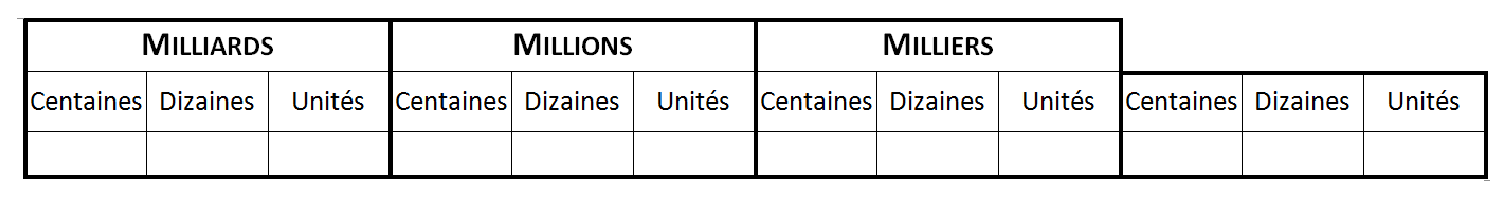
\includegraphics[scale=0.75]{tableaunumeration.eps} \\
\end{flushleft}



\bmul{2}
\exo \\
Réécrire ces nombres de façon à les rendre plus faciles à lire.\\

\noindent 12 41 56	. . . . . . . . . . . . . . . . . . . . . . . . . . . . . \\
31 25 68 9	. . . . . . . . . . . . . . . . . . . . . . . . . . . . .\\
6 54 789	. . . . . . . . . . . . . . . . . . . . . . . . . . . . .\\
7468 12 658	. . . . . . . . . . . . . . . . . . . . . . . . . . . . .\\

\columnbreak

\exo\\
Compléter les pointillées par = ou $\neq$ .\\

\noindent 041 ..... 410   \hspace*{0.5cm}  0101 ..... 1010\\
	9004 ..... 904  \hspace*{0.5cm}  004 ..... 04	\\
0102 ..... 102		\hspace*{0.5cm} 	67 ..... 670\\
1002 ..... 0120	\hspace*{0.5cm}	0300 ..... 0030\\

\emul


\bmul{2}


\exo \\

	Dans le nombre 6 083 472,\\
le chiffre des unités est : . . . . . . .\\
le chiffre des dizaines de mille est : . . . . . . .\\
le chiffre des unités de millions est : . . . . . . .\\
le nombre de centaines est : . . . . . . . . . . .\\
le nombre de centaines de mille est : . . . . . . . . . . . . .\\

\columnbreak

\exo \\
Décomposer les nombres suivants.\\

9 418 = . . . . . . . . . . . . . . . . . . . . . . . . . . . . . . \\
. . . . . . . . . . . . . . . . . . . . . . . . . . . . . . . .  \\

252 292 = . . . . . . . . . . . . . . . . . . . . . . . . . . . .\\
 . . . . . . . . . . . . . . . . . . . . . . . . . . . . . . . . . . . . . \\


\emul


\exo \\
\bmul{2}
Pour la rentrée scolaire, le directeur de l'école achète 40 livres et 4 stylos. Après avoir fait les calculs nécessaires compléter le chèque que va faire le directeur de l'école : \\


\includegraphics[scale=1]{cheque.eps} 

\columnbreak
 \begin{flushleft}
 
\includegraphics[scale=0.67]{cheque2.eps}
 \end{flushleft}
\emul


\exo\\

Je suis un nombre entier. 
\bi 
\item Mon nombre de dizaines de milliers est 5 406. 
\item Mon chiffre des centaines est la moitié de mon chiffre des unités de millions. 
\item  Mon chiffre des unités de milliers est le même que celui du nombre 49 230. 
\item  Mon chiffre des unités est égal à la différence de mon chiffre des unités de milliers et de mon chiffre des centaines. 
\item  Mon chiffre des dizaines est égal à la somme de mon chiffre des centaines et de mon chiffre des unités. 
\ei
  Qui suis-je ? \\
  
 \reponse[1]\\
 
 \newpage
 
 \vspace*{0.2cm}
 
 \exo\\
 
 Pour numéroter les pages d'un livre de un à soixante deux, \\
 \qa combien de chiffres écrit-on ?\\
 \qa combien de fois utilise-t-on le chiffre 5 ?\\
 
\noindent \reponse[3]\\

 \vspace*{0.2cm}
 
 \exo\\
  « le benjamin de la famille » \\
  
Cette famille est composée de nombres possédant deux propriétés :  
  \bi \item Ils s'écrivent avec 6 chiffres. 
    \item La somme de leurs chiffres est égale à 40. \\
   \ei
Voici deux exemples de nombres de cette famille :  \\
  \hspace*{1cm}  908 878 (9+0+8+8+7+8 = 40)  \hspace*{0.3cm} et  \hspace*{0.3cm}   753 979 (7+5+3+9+7+9 = 40)  \\

$\rightarrow$ Trouver le plus petit nombre de la famille.\\
\reponse[2]\\

 \vspace*{0.2cm}
 
 \exo\\
 
 Le \textbf{GARAM} est un jeu de logique mathématique à base d'opérations simples.\\

Remplissez chaque chaque case avec un seul chiffre de sorte que chaque ligne et chaque colonne forment une opération correcte.\\
Le résultat d'une opération verticale est un nombre à deux chiffres si deux cases suivent le symbole égal.\\

 \vspace*{0.3cm}
 
 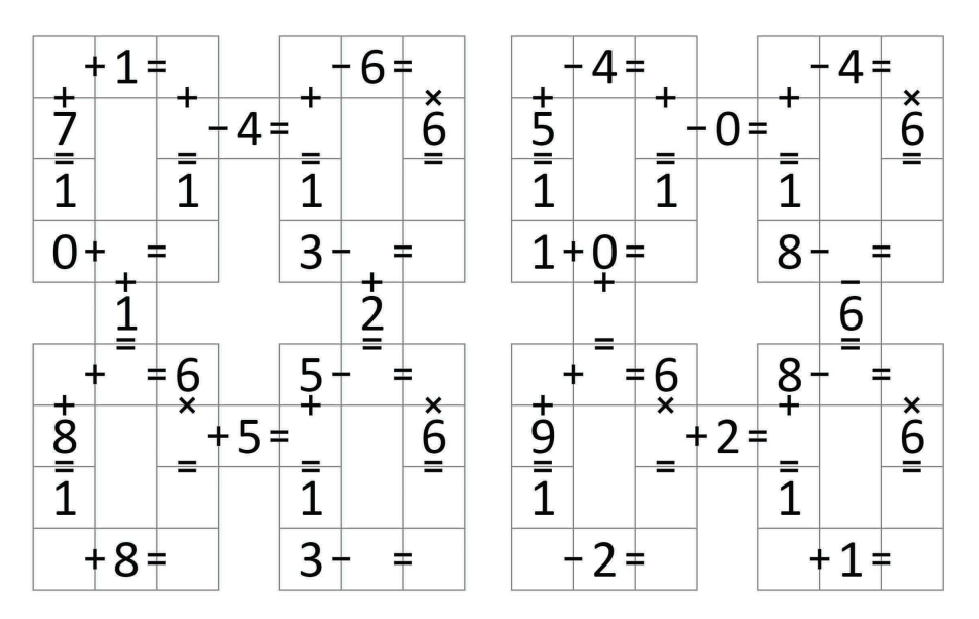
\includegraphics[scale=1]{garam1.eps} 


\end{document}
